% siminos/presentations/Haake21/Haake21.tex  pdflatex Haake21; biber Haake21
% $Author: predrag $ $Date: 2021-11-17 09:42:54 -0500 (Wed, 17 Nov 2021) $

% FROZEN                                                    2020-12-16
\date{September 22, 2021}

%  lectures/QFT20/ kittens.pdf saved as                     2020-09-27
%          ChaosBook.org/overheads/spatiotemporal/QFT20.pdf
%  started with siminos/presentations/GTmath18/GTmath18.tex 2018-03-02
%  started with siminos/presentations/KITP17/UCSB17.tex     2017-01-26
%  started with siminos/presentations/Israel16/Israel16.tex 2016-08-17
%  started with siminos/presentations/GTmap16/GTmap16.tex   2016-08-17
%  started with talks/predrag/NBI16/NBI16.tex               2016-04-25
%  started with talks/predrag/RoySoc16/RoySoc16.tex         2016-04-25

                        \newif\ifboyscout\boyscouttrue          %% comments     %%
                        \newif\ifsubmission\submissionfalse     %% internal     %%
                        \newif\ifblog\blogfalse %% section shared with blogCats %%

\input ../../inputs/layoutBeamer
\usepackage[font=scriptsize, labelfont=bf]{caption}
\usepackage[
    backend=biber,  %bibtex,
    sorting=nyt,
    %refsection=chapter,
    %citereset=chapter,
    style=numeric, %alphabetic, % %style=authoryear,
    natbib=true,
    style=phys, % aps
    biblabel= brackets, % superscript, %
    articletitle=false, % true,  % false, % aps
    %chaptertitle=true,  % aip;  % false, % aps
    pageranges = true , % aip: the full range
             % = false, % aps: only the first page being printed
    sortlocale=en_US,
    firstinits=true,
    url=false, %true,  %
    doi=false, %true,
    eprint=false
]{biblatex}
\addbibresource{../../bibtex/siminos.bib}
\setbeamerfont{footnote}{size=\tiny}
%\input ../../inputs/def % no edits, always from dasbuch/book/inputs
\input defsKittens
\input ../../inputs/defsBeamer
\renewcommand{\Ssym}[1]{{\ensuremath{m_{#1}}}}    % Boris
% \newcommand{\Ssym}[1]{{\ensuremath{s_{#1}}}}  % ChaosBook
% \newcommand{\D}{\mathcal{D}}
% \newcommand{\gd}{\mathsf{g}}

\begin{document}
\title{
{\huge chaotic field theory} %time reversal} %\catlatt}
%    \\
% {back to "amazing! I did not understand a single word!"}
}
\author{P. Cvitanovi\'c}
\author[Cvitanovi\'c]
{
  \textcolor{green!50!black}{
  {Predrag~Cvitanovi\'c
     and
    Han Liang
%   \\
%  Matt Gudorf,
  }	%\inst{1}
  }
}
\institute
{
%                    {\large Georgia Tech}
% \\
%  \inst{1}%
%\HREF{https://itsatcuny.org/calendar/chaos-and-quantum-field-theory}
%{Rutgers Mathematical Physics Seminar}
\HREF{http://ChaosBook.org/overheads/spatiotemporal}
 {ChaosBook.org/overheads/spatiotemporal}
 \\ \bigskip
    "Modern Developments in Quantum Chaos"
 \\
                Physikzentrum Bad Honnef
 }

\renewcommand{\Refl}{\ensuremath{\sigma}}             % in DasBuch
\renewcommand{\shift}{\ensuremath{r}}
\renewcommand{\hopMat}{\shift} % Aug 2021 experimental, eventually eliminate
\renewcommand{\ssp}{\ensuremath{\phi}}             % lattice site field
\renewcommand{\Xx}{\ensuremath{\mathsf{\Phi}}}      % kittens lattice field
\renewcommand{\Ssym}[1]{{\ensuremath{m_{#1}}}}    % Boris


\begin{frame}{chaotic / turbulent field theory?}
herding cats audience reviews:%
\footnote{the limiting speed for transfer of quantum-chaotic information is 1 Prozen.}
\begin{center}
  \begin{minipage}[b]{0.42\textwidth}

\bigskip
Arnd B\"acker: \\ {\footnotesize "even faster than Toma\v{z} Prosen"}

\bigskip
Martina Hentschel: \\ {\footnotesize "Amazing :)"}

\bigskip
Arnd B\"acker: \\ {\footnotesize "... maybe  I even understood \\ a single word..."}
  \end{minipage}
\qquad\quad
  \begin{minipage}[b]{0.46\textwidth}\hfill
\includegraphics[width=1.00\textwidth]{DawnBishopCats}
  \end{minipage}
\end{center}
\end{frame} %%%%%%%%%%%%%%%%%%%%%%%%%%%%%%%%%%%%%%%%%%%%%%

\begin{frame}{Nordita Quantum Chaos Symposium, 25 Nov 1988}
\begin{center}
\hfill\includegraphics[width=0.95\textheight]{IMG_3109}
\end{center}

\begin{bartlett}
     Amazing! I did not understand a single word.
\bauthor{Fritz Haake}
\end{bartlett}
\end{frame} %%%%%%%%%%%%%%%%%%%%%%%%%%%%%%%%%%%%%%%%%%%%%%

\begin{frame}
  \titlepage
\end{frame} %%%%%%%%%%%%%%%%%%%%%%%%%%%%%%%%%%%%%%%%%%%%%%

\begin{frame}{the goal was (and is)}
\vfill

\begin{center}
{\Large build
a \textcolor{blue}{chaotic field theory}
\medskip

from simple  \textcolor{blue}{chaotic blocks}
}
\end{center}

\vfill
using
\begin{itemize}
  \item
\textcolor{blue}{time invariance}
  \item
\textcolor{blue}{space invariance}
\end{itemize}
% of the defining partial differential equations
\end{frame} %%%%%%%%%%%%%%%%%%%%%%%%%%%%%%%%%%%%%%%%%%%%%%

\begin{frame}{a motivation : need a theory of {\Huge large} turbulent domains}
pipe flow close to onset of turbulence
\footnote{M.~Avila and B.~Hof, {Phys. Rev. \bf E 87} (2013)}
\begin{center}
\includegraphics[width=1.0\textwidth]{AviHof13fig4CLM}
\end{center}
we have a detailed theory of {\small \textcolor{blue}{small}} turbulent fluid cells

\bigskip

can we can we construct the \textcolor{red}{infinite} pipe by coupling small turbulent cells ?
\bigskip

\textcolor{blue}{what would that theory look like ?}
\end{frame} %%%%%%%%%%%%%%%%%%%%%%%%%%%%%%%%%%%%%%%%%%%%%%

\begin{frame}{intuition}
\begin{center}
            \begin{minipage}[c]{0.40\textwidth}\begin{center}
{\color{purple}harmonic} field theory
\bigskip

\includegraphics[width=0.35\textheight]{twodlinearEll}\\
\bigskip

{\color{blue}oscillatory eigenmodes}
            \end{center}\end{minipage}
            \hspace{2ex}
            \begin{minipage}[c]{0.46\textwidth}\begin{center}
{\color{purple}chaotic} field theory\\
\bigskip

\includegraphics[width=0.35\textheight]{twodlinearHyp}\\
\bigskip

{\color{blue}hyperbolic instabilities}
            \end{center}\end{minipage}
\end{center}
\end{frame} %%%%%%%%%%%%%%%%%%%%%%%%%%%%%%%%%%%%%%%%%%%%%%

\begin{frame}{take-home from today's talk :}
\begin{center}
            \begin{minipage}[c]{0.40\textwidth}\begin{center}
{\color{purple}harmonic} field theory
\bigskip

\includegraphics[width=0.85\textwidth]{mattressSpring}\\
{\color{blue}tight-binding} model \\ ({\color{blue}Helmholtz})
            \end{center}\end{minipage}
            \hspace{2ex}
            \begin{minipage}[c]{0.46\textwidth}\begin{center}
{\color{purple}chaotic} field theory\\
\bigskip
\bigskip
\bigskip

\includegraphics[width=1.0\textwidth]{flagellum1}\\
\bigskip

Euclidean {\color{blue}Klein-Gordon} \\ (damped {\color{blue}Poisson})
            \end{center}\end{minipage}
\end{center}
\end{frame}%%%%%%%%%%%%%%%%%%%%%%%%%%%%%%%%%%%%%%%%%%%%%%

\section[a coin toss]
 {a coin toss}

\begin{frame}{}
\begin{bartlett}{
Mephistopheles knocks at Faust's door and says, ``Du
mu{\ss}t es dreimal sagen!"
\\{\color{yellow}.}\qquad
{\scriptsize\emph{``You have to say it three times"}}
        }
\bauthor{
Johann Wolfgang von Goethe
\\{\color{yellow}.}\qquad\quad
{\em Faust I - Studierzimmer 2.~Teil}%\rf{GoetheIstuZim1806}
    }
\end{bartlett}
\vfill
\begin{enumerate}
%              \item \textcolor{gray}{\small
%what this is about
%                  }
              \item {\Large
coin toss
                  }\textcolor{gray}{\small
              \item
{\color{orange}spatio}{temporal Bernoulli}
              \item
chaotic field theory
              \item
devil is in the details
                    }
            \end{enumerate}
\end{frame}

\renewcommand{\ssp}{\ensuremath{x}}               % state space point

\begin{frame}{what we understood that day in 1988 : }
\vfill
    \begin{center}
{\huge time-evolution formulation}
    \end{center}
\vfill
\end{frame} %%%%%%%%%%%%%%%%%%%%%%%%%%%%%%%%%%%%%%%%%%%%%%

\begin{frame}{chaos} % ~~~(AKA  }
\renewcommand{\ssp}{\ensuremath{\phi}}             % lattice site field
    \begin{block}{{Bernoulli}  map} %the essence of deterministic chaos}
\begin{center}
            \begin{minipage}[c]{0.36\textwidth}\begin{center}
% ChaosBook {fig:BernPartExam}
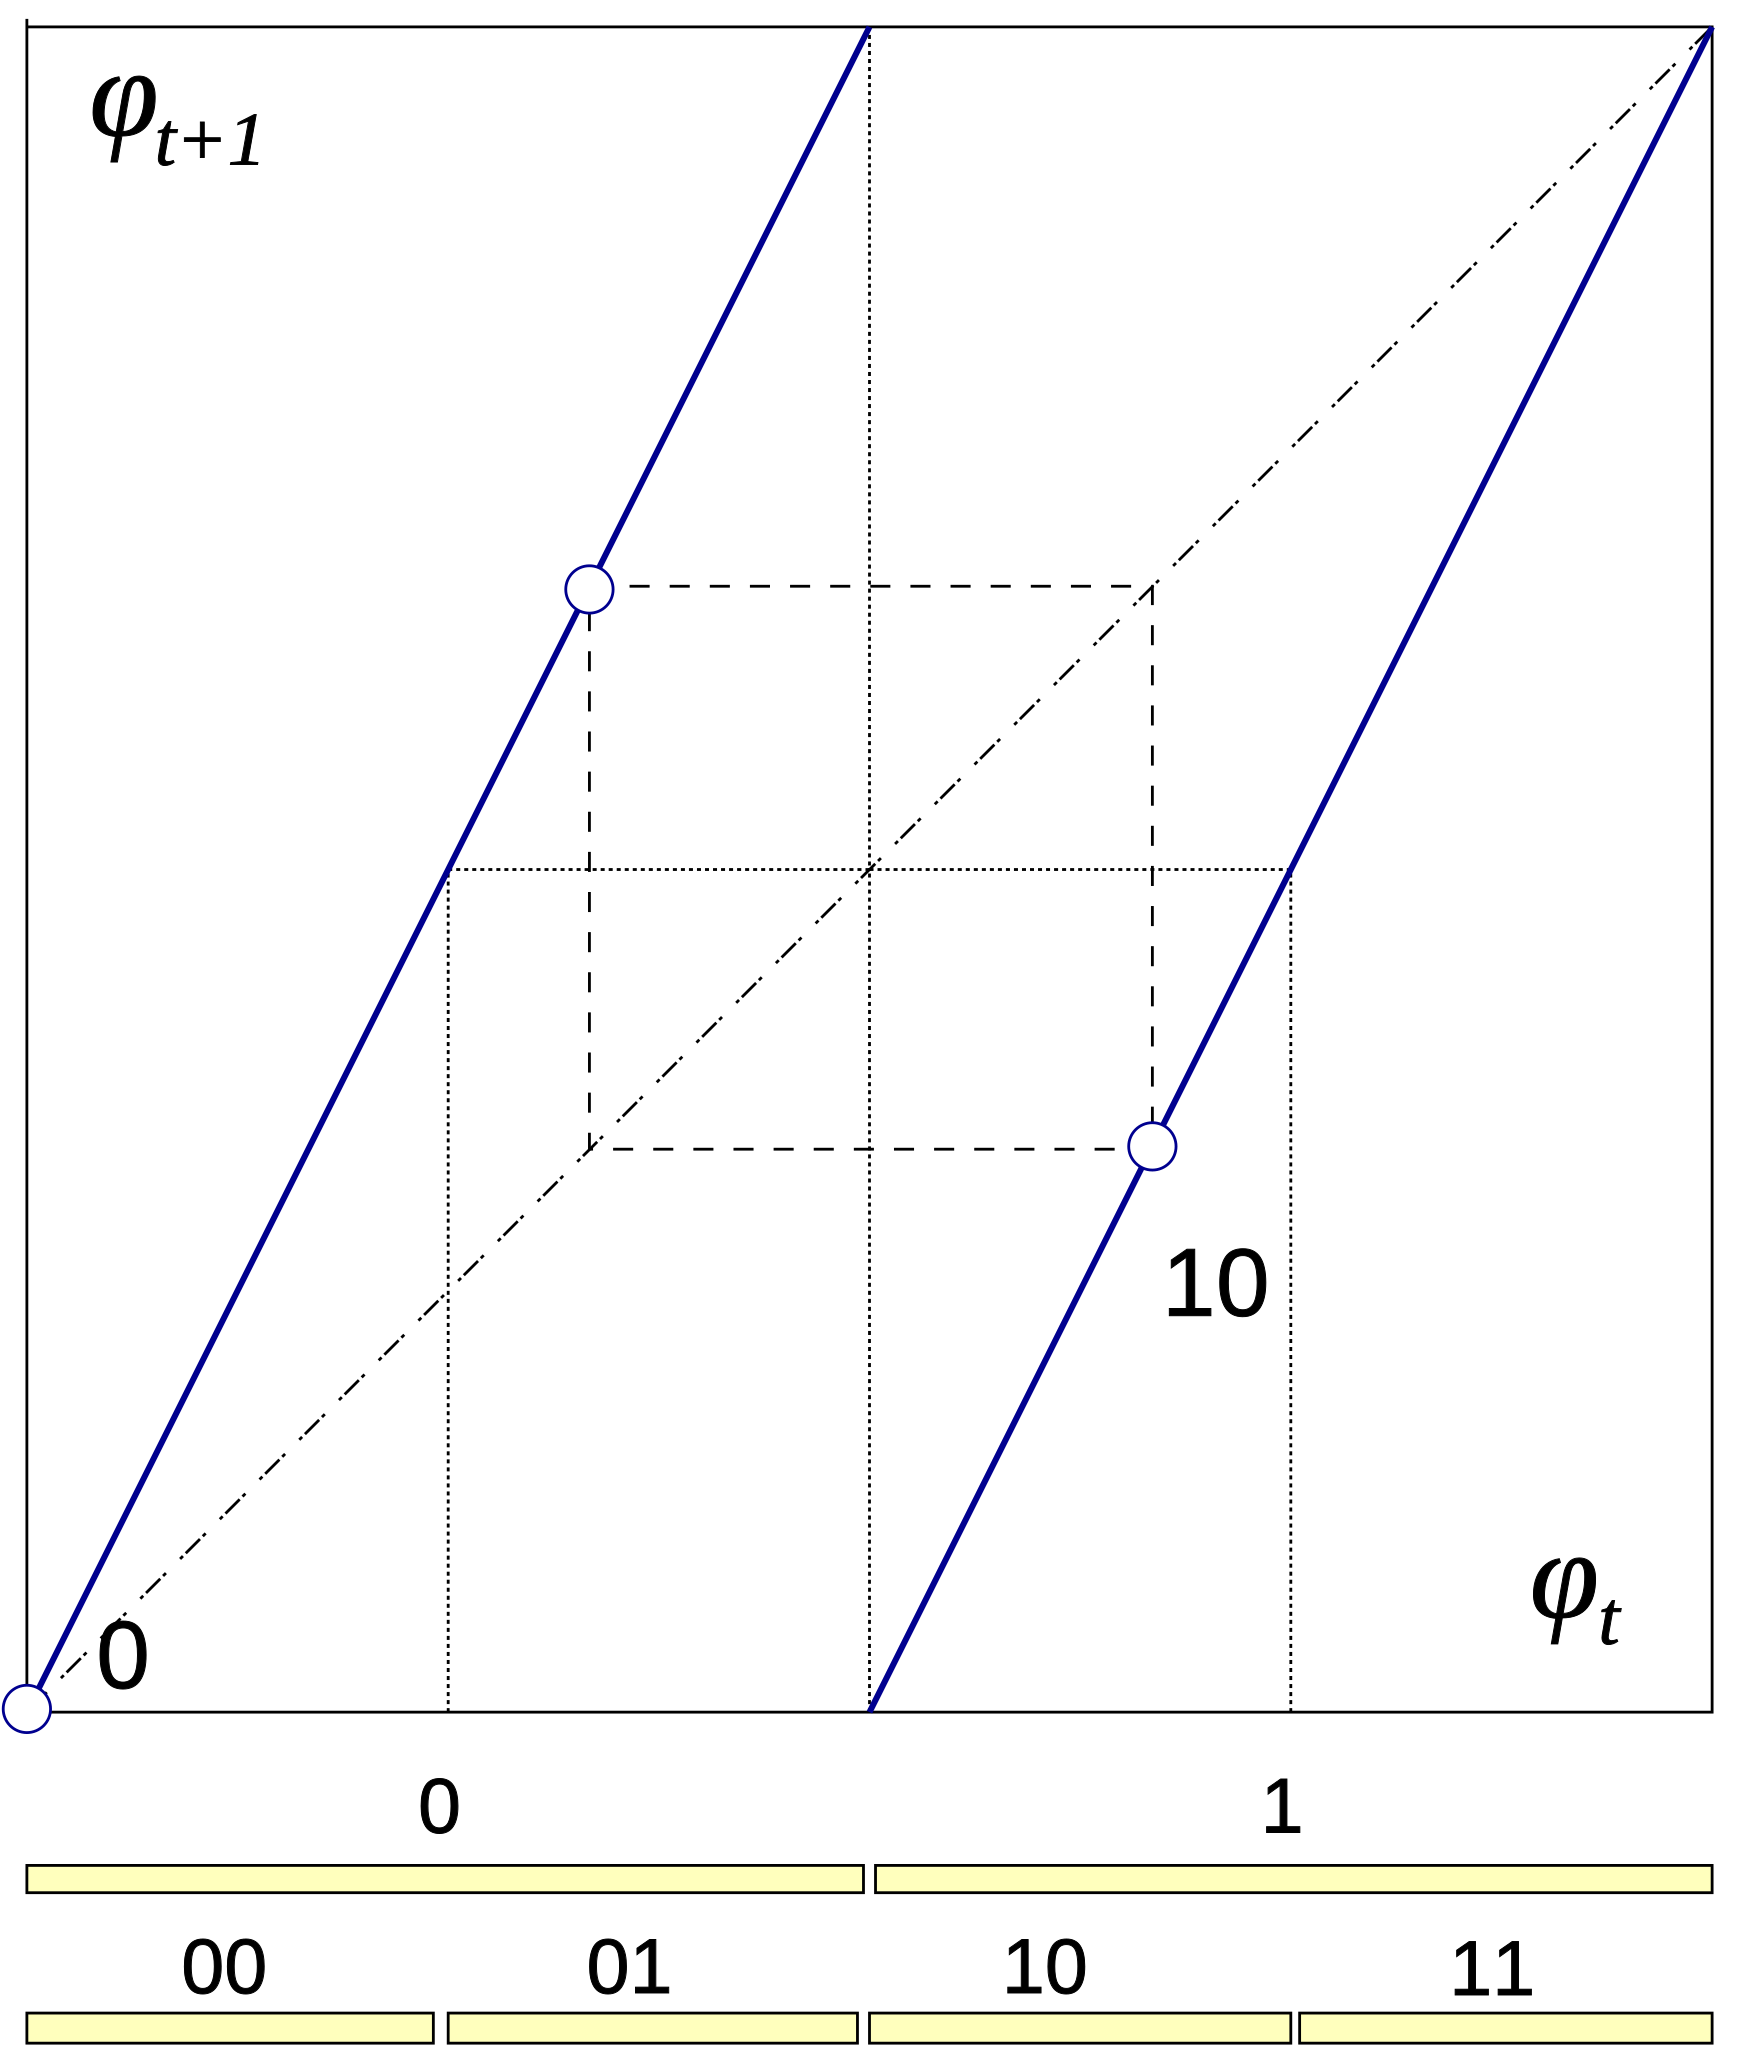
\includegraphics[width=1.0\textwidth]{BernPartKitten}
            \end{center}\end{minipage}
            \hspace{2ex}
            \begin{minipage}[c]{0.46\textwidth}\begin{center}
\[
\ssp_{\zeit+1} =
% \flow{}{\ssp_{\zeit}} =
\left\{ \begin{array}{l} %l}
        % f_0(\ssp_{\zeit}) =
        2 \ssp_{\zeit}
                             \\% \,, \quad & \ssp_{\zeit} \in \pS_0=[0,1/2) \\
        % f_1(\ssp_{\zeit}) =
        2 \ssp_{\zeit} \;\; (\mbox{mod}\;1)
                             % \,, \quad       & \ssp_{\zeit} \in \pS_1 =[1/2,1)
         \end{array}\right.
\]
            \end{center}\end{minipage}
\end{center}
%$\cl{}=2$ and 4 intervals \statesp\ partitions,

\hfill $\Rightarrow$~~~~~
fixed point \cycle{0}, 2-cycle \cycle{01}, $\cdots$
    \end{block}

\bigskip

a \HREF{https://www.random.org/coins/?num=2&cur=40-antique.aurelian}
{coin toss}

\hfill the essence of {\color{blue}deterministic chaos}
\end{frame} %%%%%%%%%%%%%%%%%%%%%%%%%%%%%%%%%%%%%%%%%%%%%%

\begin{frame}{symbolic dynamics} % what is ({mod}\;1) ?}
\renewcommand{\ssp}{\ensuremath{x}}             % lattice site field
map with a {\color{blue}`stretching' parameter $s\geq2$} :
\[
\ssp_{\zeit+1} \,=\, {s}\,\ssp_{\zeit}
\] %ee{BerStretch}

$(\mbox{mod}\;1)$ :
subtract the integer part
\(
\Ssym{\zeit+1}=\left\lfloor{s}\ssp_{\zeit}\right\rfloor
\)

\renewcommand{\ssp}{\ensuremath{\phi}}             % lattice site field
so fractional part
$\ssp_{\zeit+1}$ stays in the unit interval $[0,1)$
\[
\ssp_{\zeit+1}
= {s} \ssp_{\zeit} - \Ssym{\zeit+1}
\,,\qquad  \ssp_{\zeit}\in\pS_{\Ssym{\zeit}}
\] %ee{circ-m}
$\Ssym{\zeit}$ takes values in the ${s}$-letter alphabet
\[
\Ssym{} \in \A=\{0,1,2,\cdots,s-1\}
\] %ee{base-sAlph}
\end{frame} %%%%%%%%%%%%%%%%%%%%%%%%%%%%%%%%%%%%%%%%%%%%%%

\renewcommand{\ssp}{\ensuremath{\phi}}             % lattice site field

\begin{frame}{}
    \begin{block}{slope ${6}$ Bernoulli map}
\begin{center}
            \begin{minipage}[c]{0.32\textwidth}\begin{center}
% ChaosBook {fig:BernPartExam}
\includegraphics[width=1.0\textwidth]{fig_d_2kitten} % {fig_d_2CL18}
            \end{center}\end{minipage}
            \hspace{2ex}
            \begin{minipage}[c]{0.46\textwidth}
\(
\ssp_{\zeit+1}
= {6} \ssp_{\zeit} - \Ssym{\zeit+1}
\,,\;  \ssp_{\zeit}\in\pS_{\Ssym{\zeit}}
\)
\medskip

${6}$-letter alphabet \\
\(
\Ssym{\zeit} \in \A=\{0,1,2,\cdots,5\}
\)
            \end{minipage}
\end{center}
$6$ subintervals $\{\pS_{0},\pS_{1},\cdots,\pS_{5}\}$
    \end{block}
\end{frame} %%%%%%%%%%%%%%%%%%%%%%%%%%%%%%%%%%%%%%%%%%%%%%

\begin{frame}{what is chaos ?}
    \begin{block}{a fair dice throw}
$6$ subintervals $\{\pS_{\Ssym{\zeit}}\}$,
$6^2$ subintervals $\{\pS_{\Ssym{1}\Ssym{2}}\}, \cdots$
\begin{center}
            \begin{minipage}[c]{0.32\textwidth}\begin{center}
% ChaosBook {fig:BernPartExam}
\includegraphics[width=1.0\textwidth]{fig_d_2kitten} % {fig_d_2CL18}
            \end{center}\end{minipage}
            \hspace{2ex}
            \begin{minipage}[c]{0.46\textwidth}
each subinterval contains a periodic point,
labeled by
$\Mm=\Ssym{1}\Ssym{2}\cdots\Ssym{\cl{}}$
\bigskip

$N_\cl{} = 6^\cl{}-1$ {\color{red}unstable} orbits
            \end{minipage}
\end{center}
    \end{block}
\vfill
    \begin{block}{definition : chaos is}
positive Lyapunov $(\ln s)$ - positive entropy $(\frac{1}{\cl{}}\ln N_\cl{})$
    \end{block}
\end{frame} %%%%%%%%%%%%%%%%%%%%%%%%%%%%%%%%%%%%%%%%%%%%%%

\begin{frame}{field-theorist's chaos}
\vfill
\begin{center}
{\huge lattice formulation}
\end{center}
\vfill
\end{frame} %%%%%%%%%%%%%%%%%%%%%%%%%%%%%%%%%%%%%%%%%%%%%%

\renewcommand{\Xx}{\ensuremath{\Phi}}

\begin{frame}{lattice Bernoulli}
recast the time-evolution Bernoulli map
\[
\ssp_{\zeit+1}
= {s} \ssp_{\zeit} - \Ssym{\zeit+1}
\] %ee{circ-m}
as 1-step difference equation on the\\
{\color{orange}spatio}{\color{blue}temporal lattice}
\beq
\ssp_{\zeit} - {s}\ssp_{\zeit-1} = - \Ssym{\zeit}
\,,\qquad  \ssp_{\zeit} \in [0,1)
\ee{1stepDiffEq}
{\color{blue}field} $\ssp_\zeit$, {\color{blue}source} $\Ssym{\zeit}$ \\
on each site $\zeit$ of a
1\dmn\ lattice $\zeit\in\integers$
\bigskip
\end{frame} %%%%%%%%%%%%%%%%%%%%%%%%%%%%%%%%%%%%%%%%%%%%%%

\begin{frame}{1-dimensional lattice field theory}
 write a periodic field over \cl{}-sites Bravais cell as \\
the {\color{blue}{\lattstate}} and
the {\color{blue}symbol \brick} (sources)
\beq
{\Xx} % = \{\ssp_j\}
             = (\ssp_{\zeit+1},\cdots,\ssp_{\zeit+\cl{}})
\,,\quad
{\Mm} % = \{\Ssym{j}\}
             = (\Ssym{{\zeit+1}},\cdots,\Ssym{{\zeit+\cl{}}})
\ee{pathBern}
\begin{center}
\includegraphics[width=0.85\textheight]{HL1dLatticeStateBar1}
\end{center}

`$\Mm$' for `marching orders' ~~:~~ come here, then go there, $\cdots$
\end{frame} %%%%%%%%%%%%%%%%%%%%%%%%%%%%%%%%%%%%%%%%%%%%%%

\begin{frame}{think globally, act locally}
Bernoulli {\color{blue}condition} at every lattice site $\zeit$,
{\color{blue}local} in time
\beq
\ssp_{\zeit} - {s}\ssp_{\zeit-1} = - \Ssym{\zeit}
\ee{1stepDiffEq}
is enforced by the {\color{blue}global} equation
\beq
\left(\unit-{s}\,\hopMat^{-1}\right)\,\Xx = - \Mm
\,,
\ee{tempBern}
where $[\cl{}\!\times\!\cl{}]$ shift matrix
\beq
\hopMat_{jk}=\delta_{j+1,k}
\,,\qquad
\hopMat
=  \left(\begin{array}{ccccc}
             0    &  1    &        &   &  \cr
                  &  0    &   1    &   &  \cr
                  &       &        & \ddots &  \cr
                  &       &        & 0 & 1 \cr
             1    &       &        &   & 0
          \end{array} \right)
\ee{hopMatrix}
compares the neighbors
\end{frame} %%%%%%%%%%%%%%%%%%%%%%%%%%%%%%%%%%%%%%%%%%%%%%

\begin{frame}{think globally, act locally}
solving the {lattice Bernoulli} system
\[
\jMorb\Xx= -\Mm
\,,
\]
$[\cl{}\!\times\!\cl{}]$ {\color{blue}\jacobianOrb}
~~~~~~~~~~~~~~~
\(
\jMorb = \unit-{s}\,{\hopMat}^{-1}
\,,
\) %{tempBernFix}
\medskip

is a search for zeros of the function
\beq
F[\Xx] = \jMorb\Xx+\Mm = 0
\ee{tempFixPoint}
the entire {\color{blue}global {\lattstate}} ${\Xx}_{\Mm}$ is now
\medskip

a single {\color{blue}fixed point}
$(\ssp_1,\ssp_{2},\cdots,\ssp_{\cl{}})$

\hfill\includegraphics[width=0.12\textwidth]{hyperCube}

\hfill
in the \cl{}\dmn\ unit hyper-cube ~~~~~~~~~~~$\Xx\in[0,1)^\cl{}$
\end{frame} %%%%%%%%%%%%%%%%%%%%%%%%%%%%%%%%%%%%%%%%%%%%%%

\begin{frame}{Hill-Poincar\'e}
\vfill
\begin{center}
{\huge orbit stability}
\end{center}
\vfill
\end{frame} %%%%%%%%%%%%%%%%%%%%%%%%%%%%%%%%%%%%%%%%%%%%%%

\begin{frame}{\jacobianOrb}
solving
\[
F[\Xx]=0 \quad \mbox{ \color{blue}fixed point condition}
\]
with Newton method requires evaluation of
the $[\cl{}\!\times\!\cl{}]$
    \begin{block}{\jacobianOrb}
\[
\jMorb_{ij} =\frac{\delta F[\Xx]_i}{\delta \ssp_j}
\] %ee{jacobianOrb}
    \end{block}

what does this global \jacobianOrb\ do?
\bigskip

\begin{enumerate}
              \item
global stability of {\lattstate} \Xx, perturbed everywhere
            \end{enumerate}
\end{frame} %%%%%%%%%%%%%%%%%%%%%%%%%%%%%%%%%%%%%%%%%%%%%%

\begin{frame}{orbit stability vs. temporal stability}
\begin{block}{\jacobianOrb}
\(
\jMorb_{ij} =\frac{\delta F[\Xx]_i}{\delta \ssp_j}
\)
stability under {\color{blue}global} perturbation of the whole orbit

\hfill for \cl{} large, a huge $[d\cl{}\!\times\!d\cl{}]$ matrix
\end{block}
\begin{block}{temporal {\jacobianM}}
\(
\jMps%_\Mm
\)
propagates {\color{blue}initial} perturbation $\cl{}$ time steps

\hfill small $[d\!\times\!d]$ matrix
\end{block}
\vfill

$\jMps$ and $\jMorb$ are related by\footfullcite{Hill86}
\begin{block}{Hill's 1886 remarkable formula}
\[
|\Det\jMorb_\Mm| = |\det(\matId - \jMps_\Mm)|
%\label{catHillform}
\]
\end{block}
$\jMorb$ is {\color{red}huge}, even $\infty$\dmn\ matrix\\
$\jMps$ is {\color{red}tiny}, few degrees of freedom matrix
\end{frame} %%%%%%%%%%%%%%%%%%%%%%%%%%%%%%%%%%%%%%%%%%%%%%

\begin{frame}{field theorist's chaos}
    \begin{block}{definition : chaos is}
expanding ~~~~~~~~~~~{\color{blue}\HillDet s}
~~~~~~~~~~~$\Det\jMorb$

exponential $\sharp$~~~~~~~~{\color{blue}field configurations}
~~~~~~~$N_\cl{}$~~~
    \end{block}

\bigskip
%\hfill
the precise sense in which

a (discretized) {\color{blue}field theory}
is {\color{blue}deterministically chaotic}

\vfill
 {\color{red}\huge note} : there is no `time' in this definition
\end{frame} %%%%%%%%%%%%%%%%%%%%%%%%%%%%%%%%%%%%%%%%%%%%%%

\begin{frame}{what did Fritz not understand that day in 1988?}
\vfill
\begin{center}
{\huge \po\ theory}
\end{center}
\vfill
\end{frame} %%%%%%%%%%%%%%%%%%%%%%%%%%%%%%%%%%%%%%%%%%%%%%

\begin{frame}{volume of a \po\ neighborhood}
Ozorio de Almeida and Hannay\footfullcite{OzoHan84} 1984 :\\
$\sharp$ of periodic points is related to their temporal stability by
\begin{block}{principle of uniformity}
``periodic points of an ergodic system, counted with their natural
weighting, are uniformly dense in phase space''
\end{block}
\bigskip

where
\begin{block}{`natural weight' of \po\ {\Mm}}
\[
  \frac{1}{|\det(\unit - \jMps_{\Mm})|}
\]
\end{block}
\end{frame} %%%%%%%%%%%%%%%%%%%%%%%%%%%%%%%%%%%%%%%%%%%%%%

\begin{frame}{orbits partition state space into neighborhoods}
how come {\color{blue}\HillDet} $\Det\jMorb$ counts {\lattstate}s ?
\bigskip

`principle of uniformity' is in \footfullcite{CBgetused}
\begin{block}{\po\ theory}
known as the \HREF{http://chaosbook.org/chapters/ChaosBook.pdf\#section.27.4} {flow
conservation} sum rule  :
\beq
\sum_{{\Mm}} %\ssp_i{\in\mbox{\footnotesize Fix}\map^{\cl{}}}}
    \frac{1}{|\det (\unit - \jMps_{\Mm})|}
    \;=
\sum_{{\Mm}} %{\ssp_i{\in\mbox{\footnotesize Fix}\map^{\cl{}}}}
    \frac{1}{|\Det\jMorb_{\Mm}|}
    =1
% \label{H-OdeA_mapsOrb}
\eeq
    {\footnotesize
sum over periodic {\lattstate}s $\Xx_{\Mm}$ of period \cl{}
    }
\end{block}

\statesp\ is divided into

\hfill
{\color{blue}neighborhoods} of states of period $\cl{}$
\end{frame} %%%%%%%%%%%%%%%%%%%%%%%%%%%%%%%%%%%%%%%%%%%%%%

\begin{frame}{}
\begin{bartlett}
     Amazing! I did not understand a single word.
\bauthor{Fritz Haake 1988}
\end{bartlett}

\vfill
\begin{center}
{\huge zeta function}
\end{center}
\vfill
\end{frame} %%%%%%%%%%%%%%%%%%%%%%%%%%%%%%%%%%%%%%%%%%%%%%

\begin{frame}{\po\ theory, version (1) : counting {\lattstate}s}

\begin{block}{topological zeta function}
\[
\zetatop(z)
 \,=\,  \exp \left(-\sum_{\cl{}=1}^\infty
\frac{z^\cl{}}{\cl{}} N_\cl{}
         \right)
\] %label{BernZeta}
\end{block}
        \begin{enumerate}
              \item
weight ${1}/{\cl{}}$
as by (cyclic) translation invariance, $\cl{}$ {\lattstate}s are
equivalent
              \item
zeta function counts {\color{blue} orbits}, one per each set of equivalent
{\lattstate}s
            \end{enumerate}
\end{frame} %%%%%%%%%%%%%%%%%%%%%%%%%%%%%%%%%%%%%%%%%%%%%%

\begin{frame}{Bernoulli \tzeta}
counts {\color{blue} orbits},
one per each set of {\lattstate}s $N_\cl{}=s^{\cl{}} - 1$
\[
\zetatop(z)
 \,=\,  \exp \left(-\sum_{\cl{}=1}^\infty
\frac{z^\cl{}}{\cl{}} N_n
         \right)
\,=\,
\frac{1 -  {s}z}{1 - z}
\] %label{BernZeta}
numerator $(1 - {s}z)$ says that Bernoulli orbits are built from \\
$s$
fundamental {\color{blue}primitive} {\lattstate}s,

\hfill
the fixed points
$\{\ssp_0,\ssp_1,\cdots,\ssp_{s-1}\}$
\medskip

every other {\lattstate} is
built from their concatenations and repeats.

\vfill
\hfill {\Huge \textcolor{red}{solved!}}
\vfill

{\color{blue}this is `\po\ theory'}
\\
 And if you don't know,
\HREF{https://www.youtube.com/watch?v=_JZom_gVfuw} {now you know}

\end{frame} %%%%%%%%%%%%%%%%%%%%%%%%%%%%%%%%%%%%%%%%%%%%%%

\begin{frame}{summary : think globally, act locally}
\bigskip
the problem of enumerating and determining all global solutions stripped
to its essentials :
\bigskip
\begin{enumerate}
              \item
each solution is a zero of the global {\color{blue}fixed point} condition
\[
F[\Xx] = 0
\]
              \item
{\color{blue}global stability} :  the {\jacobianOrb}
\[
\jMorb_{ij} =\frac{\delta F[\Xx]_i}{\delta \ssp_j}
\]
              \item
{\color{blue}{\lattstate} neighborhood} : the {\HillDet}
\[
1/|\Det\jMorb|
\]

              \item
{\color{blue}zeta function} $\zetatop(z)$ : all predictions of the theory
            \end{enumerate}
\end{frame} %%%%%%%%%%%%%%%%%%%%%%%%%%%%%%%%%%%%%%%%%%%%%%


\section[a kicked rotor]
 {a kicked rotor}

\begin{frame}{}
\begin{bartlett}{
Du mu{\ss}t es dreimal sagen!
        }
\bauthor{
Mephistopheles
    }
\end{bartlett}
\vfill
\begin{enumerate}
              \item \textcolor{gray}{\small
%what this is about
%              \item
coin toss
                  }
              \item {\Large
kicked rotor
                  }\textcolor{gray}{\small
              \item
\spt\ field theory
              \item
devil is in the details
                    }
            \end{enumerate}
\end{frame} %%%%%%%%%%%%%%%%%%%%%%%%%%%%%%%%%%%%%%%%%%%%%%


\begin{frame}{building blocks od turbulence}
\begin{center}
\includegraphics[width=1.0\textwidth]{AviHof13fig4CLM}
\end{center}
have : a detailed theory of {\small \textcolor{blue}{small}} turbulent cells

\bigskip

construct : the \textcolor{red}{infinite} state by coupling turbulent
cells\footfullcite{GuBuCv17}
\vfill

\textcolor{blue}{what would that theory look like ?}
\end{frame} %%%%%%%%%%%%%%%%%%%%%%%%%%%%%%%%%%%%%%%%%%%%%%

\renewcommand{\statesp}{phase space}

\begin{frame}{example of a ``{small} turbulent cell'' : a single kicked rotor}
an electron circling an atom, subject to

a discrete time
sequence of angle-dependent kicks $F(x_{t})$

\hfill  \includegraphics[width=0.33\textwidth]{kicked-rotor}

\begin{block}{Taylor, Chirikov and Greene  standard map}
\bea
x_{t+1} - x_{t} &=& p_{t+1} \qquad  \mod 1 \continue
p_{t+1} - p_{t} &=& F(x_{t})             \nnu
\eea
\end{block}

\medskip

\hfill $\to$ {\color{red}
chaos in Hamiltonian systems}
\end{frame} %%%%%%%%%%%%%%%%%%%%%%%%%%%%%%%%%%%%%%%%%%%%%%

\begin{frame}{(1) what we understood that day in 1988?}
\vfill

\begin{center}
{\huge time-evolution formulation}
\end{center}

\vfill
\end{frame} %%%%%%%%%%%%%%%%%%%%%%%%%%%%%%%%%%%%%%%%%%%%%%

\begin{frame}{the simplest example : a cat map evolving in time}

force
\(
 F(x) = Kx
\)
{\color{blue}linear} in the displacement $x$
\,,\;
$K\in\integers$
\bea
x_{t+1} &=& x_{t}+p_{t+1} \quad\;\;  \mod 1
        \continue
p_{t+1} &=& p_{t} + K x_{t} \qquad  \textcolor{red}{\mod 1}
\nnu
\eea
 \textcolor{red}{C}ontinuous
 \textcolor{red}{A}utomorphism of the
 \textcolor{red}{T}orus, or

\begin{block}{time-evolution cat map}
a linear, area preserving map of a 2-torus onto itself
 \[
 \left[\begin{array}{c}
   \ssp_{\zeit}  \\
   \ssp_{\zeit+1}
  \end{array} \right]=
  \jMps \left[\begin{array}{c}
   \ssp_{\zeit-1}  \\
   \ssp_{\zeit}
  \end{array} \right]
 - \left[\begin{array}{c}
 0  \\
 \Ssym{\zeit}
 \end{array} \right]
\,,\qquad
\jMps = \left[
\begin{array}{cc}
0 & 1 \\
-1 & s \\
\end{array}
    \right]
 \] %\ee{PerViv:2confRepMat}

\end{block}
for integer {\color{blue}`stretching' $s=\tr{\jMps} > 2$}
the map is \\ beloved by ergodicists :\\
hyperbolic $\Rightarrow$
{\color{blue}perfect chaotic Hamiltonian dynamical system}
\end{frame} %%%%%%%%%%%%%%%%%%%%%%%%%%%%%%%%%%%%%%%%%%%%%%

\begin{frame}{a cat is literally Hooke's wild, `anti-harmonic' sister}

\begin{block}{for $s<2$ Hooke rules}
local restoring oscillations

around the sleepy z-z-z-zzz resting state
\end{block}

\begin{block}{for $s>2$ cats rule}
exponential runaway

wrapped global around a \statesp\ torus
\end{block}
\bigskip

\hfill
{\color{red}cat} is to {\color{red}chaos}
what {\color{red}harmonic oscillator} is to {\color{red}order}
\vfill
\hfill
{\color{blue}there is no more fundamental example of chaos in mechanics}
\end{frame} %%%%%%%%%%%%%%%%%%%%%%%%%%%%%%%%%%%%%%%%%%%%%%

\begin{frame}{(2) {\color{orange}spatio}{\templatt}}
\vfill
\begin{center}
{\huge lattice formulation}
\end{center}
\vfill
\end{frame} %%%%%%%%%%%%%%%%%%%%%%%%%%%%%%%%%%%%%%%%%%%%%%

\begin{frame}{cat map in lattice formulation}
replace momentum by velocity
\[
p_{t+1}=(\ssp_{t+1}  - \ssp_{t})/\Delta t
\]
obtain
 \[
 \left[\begin{array}{c}
   \ssp_{\zeit}  \\
   \ssp_{\zeit+1}
  \end{array} \right]=
  \left[
\begin{array}{cc}
0 & 1 \\
-1 & s \\
\end{array}
    \right]
    \left[\begin{array}{c}
   \ssp_{\zeit-1}  \\
   \ssp_{\zeit}
  \end{array} \right]
 - \left[\begin{array}{c}
 0  \\
 \Ssym{\zeit}
 \end{array} \right]
 \] %\ee{PerViv:2confRepMat}

temporal lattice formulation % $(\ssp_{t},\ssp_{t-1})$
is {\Large pretty}\footfullcite{PerViv} :
\begin{block}{2-step difference equation}
\[
\ssp_{t+1}  -  s \, \ssp_{t} + \ssp_{t-1}
    =
-\Ssym{t}
\] %\ee{eq:CatMapNewton1}
\end{block}
integer $\Ssym{t}$ ensures that

\hfill $\ssp_{t}$ lands in the unit interval

\bigskip
\[
\Ssym{t}\in  \A
\,,\quad \A\ = \{\mbox{finite alphabet}\}
\]
\end{frame} %%%%%%%%%%%%%%%%%%%%%%%%%%%%%%%%%%%%%%%%%%%%%%

\begin{frame}{think globally, act locally}

{\color{orange}spatio}{\templatt} at every instant $\zeit$, {\color{blue}local} in time
\[
\ssp_{t+1}  -  s \, \ssp_{t} + \ssp_{t-1}
    =
-\Ssym{t}
\] %\ee{eq:CatMapNewton1}
is enforced by the {\color{blue}global} equation
\beq
 \jMorb\,\Xx = -\Mm
\,,
\ee{catTempLatt}
where
\end{frame} %%%%%%%%%%%%%%%%%%%%%%%%%%%%%%%%%%%%%%%%%%%%%%

\begin{frame}{orbit Jacobian matrix}
\[
 \jMorb\,\Xx + \Mm= 0
\]
with
\beq
{\Xx} % = \{\ssp_j\}
             = (\ssp_{\zeit+1},\cdots,\ssp_{\zeit+\cl{}})
\,,\quad
{\Mm} % = \{\Ssym{j}\}
             = (\Ssym{{\zeit+1}},\cdots,\Ssym{{\zeit+\cl{}}})
\ee{pathBern}
a
{\color{blue}{\lattstate}}, and a {\color{blue}symbol \brick}
\bigskip

and $[\cl{}\!\times\!\cl{}]$
 {\color{blue}\jacobianOrb} \jMorb\ is
\beq
\hopMat - s\id + \hopMat^{-1}
=  \left(\begin{array}{ccccc}
            -s    &  1    &        &   & 1\cr
             1    & -s    &   1    &   &  \cr
                  &  1    &        & \ddots &  \cr
                  &       &        &-s & 1 \cr
             1    &       &        & 1 &-s
          \end{array} \right)
\ee{hopMatrix}
\end{frame} %%%%%%%%%%%%%%%%%%%%%%%%%%%%%%%%%%%%%%%%%%%%%%

\begin{frame}{think globally, act locally}
solving the {\color{orange}spatio}{\templatt}\ equation
\[
\jMorb\Xx= -\Mm
\,,
\]
with
the $[\cl{}\!\times\!\cl{}]$ matrix ~~~~~
\(
\jMorb = \hopMat - s\id + \hopMat^{-1}
\) %{tempBernFix}
\medskip

can be viewed as a search for zeros of the function
\beq
F[\Xx] = \jMorb\Xx+\Mm = 0
\ee{tempFixPoint}
where the entire {\color{blue}global {\lattstate}} ${\Xx}_{\Mm}$ is
\medskip

a single {\color{blue}fixed point}
${\Xx}_{\Mm}=(\ssp_1,\ssp_{2},\cdots,\ssp_{\cl{}})$

\hfill\includegraphics[width=0.12\textwidth]{hyperCube}

\hfill
in the \cl{}\dmn\ unit hyper-cube ~~~~~~~~~~~$\Xx\in[0,1)^\cl{}$
\end{frame} %%%%%%%%%%%%%%%%%%%%%%%%%%%%%%%%%%%%%%%%%%%%%%

\begin{frame}{what continuum theory is {\color{orange}spatio}{\templatt}\ discretization of?}
have
\begin{block}{2-step difference equation}
\[
\ssp_{t+1}  -  s \, \ssp_{t} + \ssp_{t-1}
    =
-\Ssym{t}
\] %\ee{eq:CatMapNewton1}
\end{block}
discrete lattice
\begin{block}{Laplacian in $1$ dimension}
\[
\ssp_{t+1} - 2\ssp_{t} + \ssp_{t-1}
     =
\Box\,\ssp_t
\]
\end{block}
\medskip

so {\color{orange}spatio}{\templatt}\ is an (anti)oscillator chain, known as
\begin{block}{$d=1$ Klein-Gordon (or damped Poisson) equation (!)}
\[
 (-\Box + {\mu}^2)\,\ssp_{t} = \m_t
\,, \qquad
{\mu}^2= s-2
\] %\ee{LinearConn}
\end{block}
\vfill\hfill
\textcolor{red}{did you know that a cat map can be so cool?}
\end{frame} %%%%%%%%%%%%%%%%%%%%%%%%%%%%%%%%%%%%%%%%%%%%%%

\begin{frame}{what did Fritz not understand that day in 1988?}

{\color{orange}spatio}{\templatt} topological zeta function
is the generating function that counts {\color{blue}orbits}
\medskip

substituting the {\color{blue}\HillDet} count of periodic {\lattstate}s
\[
N_n=|\Det\jMorb|
\]
into the
{topological} zeta func\-tion
\[
\zetatop(z)
  =   \exp \left(
    -\sum_{n=1} \frac{z^n}{n} N_n
    \right)
\]%\label{perOrbits:Isola90-13}
leads to the elegant explicit formula\footfullcite{Isola90}
\[
\zetatop(z)
 =  \frac{1 - s z + z^2}
         {1 - 2 z + z^2}
\]%\label{perOrbits:Isola90-13}


\vfill\hfill
{\Huge \textcolor{red}{solved!}}
\end{frame} %%%%%%%%%%%%%%%%%%%%%%%%%%%%%%%%%%%%%%%%%%%%%%

\begin{frame}{that's it! for spacetime of $1$ dimension}
lattice Klein-Gordon equation
    {\Huge
\[
  (-\Box + {\mu}^2)\,\ssp_{t} = \m_t
%    \,, \qquad
\] %\ee{LinearConn}
    }
\hfill solved completely and analytically!
\end{frame} %%%%%%%%%%%%%%%%%%%%%%%%%%%%%%%%%%%%%%%%%%%%%%

\section[\catlatt]
 {\catlatt}
\label{s:catLatt}

\begin{frame}{}
\begin{bartlett}{
Du mu{\ss}t es dreimal sagen!
        }
\bauthor{
Mephistopheles
    }
\end{bartlett}
\vfill
\begin{enumerate}
              \item \textcolor{gray}{\small
%what this is about
%              \item
coin toss
              \item
kicked rotor
                  }
              \item {\Large
chaotic field theory
                  }\textcolor{gray}{\small
              \item
devil is in the details
                    }
            \end{enumerate}
\end{frame} %%%%%%%%%%%%%%%%%%%%%%%%%%%%%%%%%%%%%%%%%%%%%%

\begin{frame}{Euclidean lattice field theory}
    \begin{block}{scalar \emph{field} $\ssp(x)$}
 evaluated on lattice points
%\bigskip

\begin{center}
            \begin{minipage}[c]{0.32\textwidth}\begin{center}
\includegraphics[width=0.95\textwidth]{MunWal00lattice}
            \end{center}
% 3$d$ lattice
% \label{fig:MunWal00lattice}
            \end{minipage}
            \hspace{2ex}
            \begin{minipage}[c]{0.46\textwidth}
$\ssp_z
=
\ssp(x)$
\\
$
x = az= \mbox{lattice point}$
\\
$
z \in \integers^d/\speriod{}^d
$
%\ee{LattField}
            \end{minipage}
\end{center}
a periodic point per each unit cell
    \end{block}
\footfullcite{MunWal00}
\end{frame} %%%%%%%%%%%%%%%%%%%%%%%%%%%%%%%%%%%%%%%%%%%%%%

\begin{frame}{Discretization of a $1d$ field theory}
    \begin{block}{scalar \emph{field} $\ssp(x)$ evaluated on lattice points}

\begin{center}
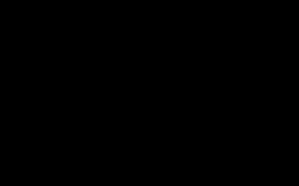
\includegraphics[width=0.55\textwidth]{LC21FieldConfig}

\bigskip
            \begin{minipage}[c]{0.42\textwidth}
periodic field $\ssp(\zeit)$
\\
is a function of
\\
continuous coordinate $\zeit$
            \end{minipage}
            \hspace{2ex}
            \begin{minipage}[c]{0.42\textwidth}
corresponding discretized period-$5$ {\lattstate}
\\
$\Xx=\cycle{\ssp_0 \ssp_1 \ssp_2 \ssp_3 \ssp_4}$,
            \end{minipage}
\end{center}
    \end{block}
Horizontal: $\zeit$ coordinate, lattice sites marked by
\\
dots, labelled by $\zeit\in\integers$

\medskip
the value of the discretized field $\ssp_\zeit$ is plotted as
\\
a bar centred at lattice site $\zeit$
\end{frame} %%%%%%%%%%%%%%%%%%%%%%%%%%%%%%%%%%%%%%%%%%%%%%

\begin{frame}{think globally, act locally}
    \begin{center}
\includegraphics[width=0.85\textwidth]{globalLocal}
    \end{center}
for each symbol array \Mm, a periodic {\lattstate} $\Xx_\Mm$
\end{frame} %%%%%%%%%%%%%%%%%%%%%%%%%%%%%%%%%%%%%%%%%%%%%%

\begin{frame}{example : Euclidean {$\phi^4$} theory}
    \begin{block}{lattice action}
\bea
S &=&
\sum_x a^d \left\{ \frac{1}{2} \sum_{i =1}^d
(\partial_{\mu}\ssp(x))^2 + \frac{\mu^2}{2}\ssp(x)^2 + \frac{g}{4!}\ssp(x)^4
\right\}
\continue
 &=&
\sum_{z,z'} \frac{1}{2}\left\{
\ssp_z\left(-\Box + \mu^2\right)_{zz'}\ssp_{z'}
\right\}
 + \sum_{z}\frac{g}{4!}\ssp_z^4
\,.
%\label{MunWal00freeAct}
\eea
    \end{block}
\end{frame} %%%%%%%%%%%%%%%%%%%%%%%%%%%%%%%%%%%%%%%%%%%%%%

\begin{frame}{examples : 1$d$ lattice field theories}

{\color{orange}spatio}temporal lattice field theory
\bea
\ssp_{\zeit+1}  - S'[\ssp_{\zeit}] + \ssp_{\zeit-1}
    &=&
-\Ssym{\zeit}
%\,,\qquad  \ssp_{\zeit} \in [0,1)
%\label{LC21:1dTempFT}
\eea

{\color{orange}spatio}temporal  Bernoulli
\bea
\ssp_{\zeit+1} - {s}\,\ssp_{\zeit}
    \qquad\quad\;
    &=&
- \Ssym{\zeit}
%\,,\qquad  \ssp_{\zeit} \in [0,1)\,,
%\label{LC21:1dBernLatt}    % labelled {1stepDiffEq} elsewhere
\eea

{\color{orange}spatio}{\templatt}
\bea
\ssp_{\zeit+1}  -  \,{s}\,\ssp_{\zeit} + \ssp_{\zeit-1}
    &=&
-\Ssym{\zeit}
%\,,\qquad  \ssp_{\zeit} \in [0,1)
\eea %    \continue %\label{LC21:1dTemplatt}\\
{\color{orange}spatio}{\henlatt}
\bea
\ssp_{\zeit+1} - {a}\,\ssp_{\zeit}^2 +\ssp_{\zeit-1}
    &=&
-\Ssym{\zeit}
%\,,\qquad  \Ssym{\zeit}=2
\eea %    \continue %\label{LC21:1dHenlatt}\\
{\color{orange}spatio}temporal {$\phi^4$} theory
\bea
\ssp_{\zeit+1} - \frac{g}{3!}\ssp_{\zeit}^3 +\ssp_{\zeit-1}
    &=&
-\Ssym{\zeit}
%\,,
%\label{LC21:1dPhi4}
\eea
\end{frame} %%%%%%%%%%%%%%%%%%%%%%%%%%%%%%%%%%%%%%%%%%%%%%

\begin{frame}{herding cats in $d$ spacetime dimensions : `\catlatt'}
%\begin{center}
%\hfill\includegraphics[width=0.55\textwidth]{spatiotempCat}
\hfill\includegraphics[width=0.55\textwidth]{DawnBishopCats}
%\end{center}
\end{frame} %%%%%%%%%%%%%%%%%%%%%%%%%%%%%%%%%%%%%%%%%%%%%%

\begin{frame}{\catlatt}
consider
a 1 {\color{blue}spatial} dimension lattice, with field
$\ssp_{nt}$ \\
(the angle of a kicked
rotor ``particle'' at instant $t$, at site $n$)
\begin{block}{require}
\begin{itemize}
\item  each site couples to
its nearest neighbors $\ssp_{n\pm1,t}$
\item  invariance under
spatial translations
\item  invariance under spatial reflections
\item  invariance under the space-time exchange
\end{itemize}
\end{block}

\bigskip

Gutkin \& Osipov\footfullcite{GutOsi15} obtain\footfullcite{GHJSC16}${}^,$\footfullcite{CL18}
\begin{block}{2\dmn\ coupled cat map lattice}
\[
\ssp_{n,t+1} + \ssp_{n,t-1} - 2s \, \ssp_{n t} + \ssp_{n+1,t} + \ssp_{n-1, t}
     =-\Ssym{n t}
\] %\ee{eq:CatMapNewton2}
\end{block}
\end{frame} %%%%%%%%%%%%%%%%%%%%%%%%%%%%%%%%%%%%%%%%%%%%%%

\begin{frame}{herding cats : a discrete Euclidean space-time field theory}
write the spatial-temporal differences as discrete derivatives
\begin{block}{Laplacian in %$d=1$ and
              $d=2$ dimensions}
%\(
%\Box\,\ssp_t \;\;\,=\, \ssp_{t+1} - 2\ssp_{t} + \ssp_{t-1}
%\)\\
\(
\Box\,\ssp_{nt} \,=\, \ssp_{n,t+1} + \ssp_{n,t-1}
- 4 \, \ssp_{nt} + \ssp_{n+1,t} + \ssp_{n-1, t}
\)\\
~~~~{\scriptsize subtract 2\dmn\ coupled cat map lattice equation}\\
\(
-\Ssym{n t}
 =
\ssp_{n,t+1} + \ssp_{n,t-1} - 2s \, \ssp_{n t} + \ssp_{n+1,t} + \ssp_{n-1, t}
\) %\ee{eq:CatMapNewton2}
\end{block}

\bigskip

{\color{blue}cat herd} is thus governed by the law of
\begin{block}{$d$\dmn\ \catlatt}
\[
 (-\Box + {\mu}^2)\,\ssp_{z} = \m_z
\,, \qquad
{\mu}^2= d(s-2)
\] %\ee{LinearConn}

\medskip

\end{block}

\bigskip

where
\(
  \ssp_{z} \in [0,1)
    \,, \quad
  \Ssym{z} \in \A
    \mbox{  and  }
  z\in \integers^{d}
\) = integer lattice
\end{frame} %%%%%%%%%%%%%%%%%%%%%%%%%%%%%%%%%%%%%%%%%%%%%%

\begin{frame}{discretized linear PDE}
\begin{block}{$d$\dmn\ \catlatt}
{\Large
\[
 (-\Box + {\mu}^2)\,\ssp_{z} = \m_z
\] %\ee{LinearConn}
}
\end{block}

\bigskip

is linear and known as
\begin{itemize}
\item {\color{blue}tight-binding} model or {\color{blue}Helmholtz} equation \\
if stretching is weak, $s<2$ \\
 $[$oscillatory sine, cosine solutions]
\item
Euclidean {\color{blue}Klein-Gordon} or (damped {\color{blue}Poisson})\\
if stretching is strong, $s>2$ \\
 $[$hyperbolic sinches, coshes, `{\color{blue}mass}' ${\mu}^2=d(s-2)$]
\end{itemize}
\medskip

nonlinearity is hidden in the `sources'
\[
  \Ssym{z} \in \A
    \mbox{  at lattice site  }
  z\in \integers^{d}
\]
\end{frame} %%%%%%%%%%%%%%%%%%%%%%%%%%%%%%%%%%%%%%%%%%%%%%

\begin{frame}{spring mattress vs field of rotors}
\begin{center}
            \begin{minipage}[c]{0.40\textwidth}\begin{center}
traditional field theory
\bigskip

\includegraphics[width=0.85\textwidth]{mattressSpring}\\
{\color{blue}Helmholtz}
            \end{center}\end{minipage}
            \hspace{2ex}
            \begin{minipage}[c]{0.46\textwidth}\begin{center}
chaotic field theory\\
\bigskip
\bigskip
\bigskip

\includegraphics[width=1.0\textwidth]{flagellum1}\\
\bigskip

damped {\color{blue}Poisson}
            \end{center}\end{minipage}
\end{center}
\end{frame} %%%%%%%%%%%%%%%%%%%%%%%%%%%%%%%%%%%%%%%%%%%%%%

\begin{frame}{our song of chaos has been sang -- what next ?}
\begin{enumerate}
              \item \textcolor{gray}{\small
%what this is about
%              \item
coin toss
              \item
kicked rotor
              \item
\catlatt
                  }
              \item {\Large
devil is in the details
%                  }\textcolor{gray}{\small
%              \item
%devil is in the details
                    }
            \end{enumerate}
\end{frame} %%%%%%%%%%%%%%%%%%%%%%%%%%%%%%%%%%%%%%%%%%%%%%

\begin{frame}{Zetastan : lost in translation}
\begin{center}
\hfill\includegraphics[width=0.90\textwidth]{../kittens/lattLitClip1}
\end{center}
\end{frame} %%%%%%%%%%%%%%%%%%%%%%%%%%%%%%%%%%%%%%%%%%%%%%

\begin{frame}{Zetastan : lost, but not alone}
\begin{center}
\hfill\includegraphics[width=0.90\textwidth]{../kittens/lattLitClip2}
\end{center}
\end{frame} %%%%%%%%%%%%%%%%%%%%%%%%%%%%%%%%%%%%%%%%%%%%%%

\section[devil is in the details]
 {devil is in the details}
\label{s:byeDynamics}

\begin{frame}{devil is in the details}
\vfill
\begin{center}
{\huge symmetry reduction}
\end{center}
\vfill
\end{frame} %%%%%%%%%%%%%%%%%%%%%%%%%%%%%%%%%%%%%%%%%%%%%%

\begin{frame}{\catlatt\ : a strong coupling field theory}

%2020-09-05
%\subsection{Symmetries of the integer lattice}
%\label{s:lattSymm}
\begin{block}{\catlatt\ symmetries :}
translations $\circ$ time-reversal $\circ$ spatial reflections
\end{block}
point-group of the square lattice:
\\ rotations by $\pi/2$
\\ reflections across axes  and diagonals,
\[ %beq
\Dn{4} = \{
1, \shift, \shift^2, \shift^3,
\Refl, \Refl_{1},
\Refl_{2},\Refl_{3}
\}
\,.
\] %\ee{eq:C4v}
international crystallographic notation\footfullcite{Dresselhaus07},
\\
the square lattice space group $p4mm$.

\bigskip
{\color{red}not} a traditional \\
{\color{blue}spatially
weakly coupled} lattice model\footfullcite{BunSin88}
%\bigskip
%\vfill
\end{frame} %%%%%%%%%%%%%%%%%%%%%%%%%%%%%%%%%%%%%%%%%%%%%%

\begin{frame}{symmetries of a square lattice unit cell}
%%%%%%%%%%%%%%%%%%%%%%%%%%%%%%%%%%%%%%%%%%%%%%%%%%%%%%%%%%%%%%%%%%
% PC 2021-08-05:  from ChaosBook book/figs/D3.tex, D3.tex
\begin{center}
  \begin{minipage}[b]{0.39\textwidth}\begin{center}
  \setlength{\unitlength}{1.00\textwidth}
  \begin{picture}(1,0.94270725)%
    \setlength\tabcolsep{0pt}%
    \put(0,0){\includegraphics[width=\unitlength,page=1]{D4}}%
    \put(0.11589164,0.70318699){\color[rgb]{1,1,1}\makebox(0,0)[lt]{\smash{{\Large 2}}}}%
    \put(0.11465857,0.11853823){\color[rgb]{1,1,1}\makebox(0,0)[lt]{\smash{{\Large 3
    }}}}%
    \put(0,0){\includegraphics[width=\unitlength,page=2]{D4}}%
    \put(0.69662672,0.11848457){\color[rgb]{1,1,1}\makebox(0,0)[lt]{\smash{{\Large 0}}}}%
    \put(0.69785979,0.70163221){\color[rgb]{1,1,1}\makebox(0,0)[lt]{\smash{{\Large 1}}}}%
    \put(0.48887673,0.58974203){\color[rgb]{0.1372549,0.12156863,0.1254902}\makebox(0,0)[lt]{\smash{$\shift_1$}}}%
    \put(0,0){\includegraphics[width=\unitlength,page=3]{D4}}%
    \put(0.24073374,0.49925981){\color[rgb]{0.1372549,0.12156863,0.1254902}\makebox(0,0)[lt]{\smash{$\shift_2$}}}%
    \put(0.33991763,0.28480816){\color[rgb]{0.1372549,0.12156863,0.1254902}\makebox(0,0)[lt]{\smash{$\shift_3$}}}%
    \put(0.95378545,0.34914366){\color[rgb]{0.1372549,0.12156863,0.1254902}\makebox(0,0)[lt]{\smash{$\Refl_1$}}}%
    \put(0.87112523,0.73973783){\color[rgb]{0.1372549,0.12156863,0.1254902}\makebox(0,0)[lt]{\smash{$\Refl_2$}}}%
    \put(0.50562029,0.87631462){\color[rgb]{0.1372549,0.12156863,0.1254902}\makebox(0,0)[lt]{\smash{$\Refl_3$}}}%
    \put(0.11826698,0.87765494){\color[rgb]{0.1372549,0.12156863,0.1254902}\makebox(0,0)[lt]{\smash{$\Refl$}}}%
    \put(0,0){\includegraphics[width=\unitlength,page=4]{D4}}%
  \end{picture}
  \end{center} \end{minipage}
  \end{center}
%  \caption{\label{fig:D3D4}
% Dihedral group \Dn{3}: \Dn{4}:

4 rotations $\shift_j$, 4 shift-reflections
$\Refl_k$ of dihedral group
\[ %beq
\Dn{4} = \{
1, \shift, \shift^2, \shift^3,
\Refl, \Refl_{1},
\Refl_{2},\Refl_{3}
\}
\] %\ee{eq:C4v}
%even reflection axes dashed, odd reflections full line
overly the square onto itself.

They also tile it with  the $8$ copies $\pSRed_\ell$ of
\\
the {\color{blue}fundamental domain} (the shaded wedge)
\end{frame} %%%%%%%%%%%%%%%%%%%%%%%%%%%%%%%%%%%%%%%%%%%%%%

\begin{frame}{retreat to : 1$d$ lattice field theories}

{\color{orange}spatio}{\templatt}
\bea
\ssp_{\zeit+1}  -  \,{s}\,\ssp_{\zeit} + \ssp_{\zeit-1}
    &=&
-\Ssym{\zeit}
%\,,\qquad  \ssp_{\zeit} \in [0,1)
\eea %    \continue %\label{LC21:1dTemplatt}\\
{\color{orange}spatio}{\henlatt}
\bea
\ssp_{\zeit+1} - {a}\,\ssp_{\zeit}^2 +\ssp_{\zeit-1}
    &=&
-\Ssym{\zeit}
%\,,\qquad  \Ssym{\zeit}=2
\eea %    \continue %\label{LC21:1dHenlatt}\\
{\color{orange}spatio}temporal {$\phi^4$} theory
\bea
\ssp_{\zeit+1} - \frac{g}{3!}\ssp_{\zeit}^3 +\ssp_{\zeit-1}
    &=&
-\Ssym{\zeit}
%\,,
%\label{LC21:1dPhi4}
\eea
\end{frame} %%%%%%%%%%%%%%%%%%%%%%%%%%%%%%%%%%%%%%%%%%%%%%

\begin{frame}{orbit Jacobian (Hill, Hessian, ...)  matrix}
each {\lattstate} has its own
\beq
\jMorb[\Xx] =
\left(\begin{array}{cccccccc}
%\begin{pmatrix}
-{s}_{0} & 1 & 0 & 0 & \cdots & 0 & 0 & 1 \\
1 & -{s}_{1} & 1 & 0 & \cdots & 0 & 0 & 0 \\
0 & 1 & -{s}_{2} & 1 & \cdots & 0 & 0 & 0 \\
\vdots & \vdots & \vdots & \vdots & \ddots & \vdots & \vdots & \vdots \\
0 & 0 & 0 & 0 & \cdots & 1 & -{s}_{\cl{}-2} & 1 \\
1 & 0 & 0 & 0 & \cdots & 0 & 1 & -{s}_{\cl{}-1}
%\end{pmatrix}
          \end{array} \right)
\,,
\ee{jMorb1dFT} %was {jMorb1dField}, {PCJiKoKr20(8)}
{\color{orange}stretching factor} ${s}_{\zeit}= S''[\ssp_{\zeit}]$ is
\\
function of the site field $\ssp_\zeit$ for the
given \lattstate\ $\Xx$

\bigskip
  \begin{enumerate}
              \item
can compute {\color{blue}\HillDet} $\Det\jMorb$
              \item
Hill-Lindstedt-Poincar\'e : \\
all calculations should be done
on reciprocal lattice
              \item
toolbox : discrete Fourier transforms, irreps of \Dn{n}
   \end{enumerate}
\end{frame} %%%%%%%%%%%%%%%%%%%%%%%%%%%%%%%%%%%%%%%%%%%%%%

\begin{frame} {Symmetries of 1\dmn\ lattices}
There are only two \HREF{https://en.wikipedia.org/wiki/Line_group}
{1\dmn\ space groups}  $\Group$:
\\
$p1$ \emph{infinite cyclic
group}  \Cn{\infty} of all lattice translations,
\beq
\Cn{\infty}
    =       \{
\cdots, \shift_{-2}, \shift_{-1},
        1,
        \shift_{1}, \shift_{2}, \shift_{3}, \cdots
             \}
\label{C_infty}
\eeq

$p1m$, the \emph{infinite dihedral group} $\Dn{\infty}$  of all
translations and reflections\footfullcite{KiLePa03},
\beq
  \Dn{\infty} = \{
\cdots, \shift_{-2},\Refl_{-2}, \shift_{-1},\Refl_{-1},
        1,\Refl,
        \shift_{1},\Refl_{1}, \shift_{2},\Refl_{2}, \cdots
             \}
%\,.
\ee{LC21D_infty}
group multiplication
$\LieEl_i\LieEl_j$
\beq
\begin{tabular}{c|cc}
%\Dn{\infty} &\shift_j        &\Refl_j\\\hline
            &$\shift_j$        &$\Refl_j$\\\hline
$\shift_i$  &$\shift_{i+j}$     &$\Refl_{j-i}$\\
$\Refl_i$   &$\Refl_{i+j}$     &$\shift_{j-i}$
\end{tabular}
\ee{eq:DinftyMultTab}
either adds up translations,
\\
or shifts and then reverses their direction
\end{frame} %%%%%%%%%%%%%%%%%%%%%%%%%%%%%%%%%%%%%%%%%%%%%%

\begin{frame} {Symmetries of 1\dmn\ Bravais sublattices}
\emph{Bravais cell} of \emph{period} \cl{} : given by vector
$\mathbf{a}$ of length \cl{}

\emph{Bravais  sublattice} generated by translations
\[
  \shift_{j}\to\shift_{j\mathbf{a}}
\]
symmetry : translation subgroup of $\Cn{\infty}$
\beq
H_{\mathbf{a}} = \{ \cdots, \shift_{-2 \mathbf{a}}, \shift_{-\mathbf{a}},
1, \shift_{\mathbf{a}}, \shift_{2 \mathbf{a}}, \cdots\}
\,,
\ee{H(n)subgroup}
and
% a tiling of the lattice $\integers$ by a generic
% {\lattstate} tile of length \cl{}
\[
  \shift_{j}\to\shift_{j\mathbf{a}}
\,,\qquad
    \Refl\to \Refl_{k}
  \quad
     0\leq{k}<\cl{}
\,,
\]
symmetry :  $\cl{}$ infinite dihedral subgroups of $\Dn{\infty}$
\beq
H_{\mathbf{a},k} = \{
\cdots, \shift_{-2 \mathbf{a}}, \Refl_{k}\shift_{-2 \mathbf{a}},
        \shift_{-\mathbf{a}}, \Refl_{k}\shift_{-\mathbf{a}},
        1,                    \Refl_{k},
        \shift_{\mathbf{a}},  \Refl_{k}\shift_{\mathbf{a}},
        \shift_{2\mathbf{a}},\Refl_{k}\shift_{2\mathbf{a}}, \cdots
             \}
\,,
\ee{H(n,k)subgroup}
{Bravais cell} of period \cl{},
\\
with reflection
across a symmetry point shifted $k$ 1/2 steps
\end{frame} %%%%%%%%%%%%%%%%%%%%%%%%%%%%%%%%%%%%%%%%%%%%%%

\begin{frame} {$\Dn{\infty}$ orbit of a generic {\lattstate}}
%%%%%%%%%%%%%%%%%%%%%%%%%%%%%%%%%%%%%%%%%%%%%%%%%%%%%
\begin{center}
  \begin{minipage}[b]{0.17\textwidth}\begin{center}
{(1)}~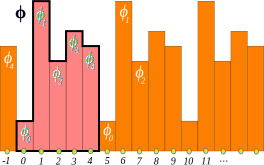
\includegraphics[width=\textwidth]{1dLatStatC_5_0}
\\
{($\shift_1$)}~\includegraphics[width=\textwidth]{1dLatStatC_5_1}
\\
{($\shift_2$)}~\includegraphics[width=\textwidth]{1dLatStatC_5_2}
\\
{($\shift_3$)}~\includegraphics[width=\textwidth]{1dLatStatC_5_3}
\\
{($\shift_4$)}~\includegraphics[width=\textwidth]{1dLatStatC_5_4}
  \end{center}\end{minipage}
\qquad\quad
  \begin{minipage}[b]{0.17\textwidth}\begin{center}
{($\Refl$)}~\includegraphics[width=\textwidth]{1dLatStatC_5_s0}
\\
{($\Refl_1$)}~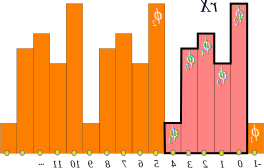
\includegraphics[width=\textwidth]{1dLatStatC_5_s1}
\\
{($\Refl_2$)}~\includegraphics[width=\textwidth]{1dLatStatC_5_s2}
\\
{($\Refl_3$)}~\includegraphics[width=\textwidth]{1dLatStatC_5_s3}
\\
{($\Refl_4$)}~\includegraphics[width=\textwidth]{1dLatStatC_5_s4}

  \end{center} \end{minipage}
  \end{center}
%  \caption{\label{fig:1dLatStatC_5}
% (1)
{\lattstate}
% \refeq{1dLattStatC_n}
\(\Xx=\cycle{\ssp_0 \ssp_1 \ssp_2 \ssp_3 \ssp_4}\),
no reflection symmetry
\\
 translation group $H_{5}$ invariant

\Dn{\infty}-orbit is isomorphic to $\Dn{5}$ : $10$ distinct {\lattstate}s
\end{frame} %%%%%%%%%%%%%%%%%%%%%%%%%%%%%%%%%%%%%%%%%%%%%%

\begin{frame} {4 kinds of Bravais lattice states}
\begin{center}
{$(n)$}
\includegraphics[width=0.40\textwidth]{HL1dLatticeStateBar1}\quad~~~
{$(o)$}
\includegraphics[width=0.40\textwidth]{HL1dLatticeStateBar2}
\\ %~~~
{$(ee)$}
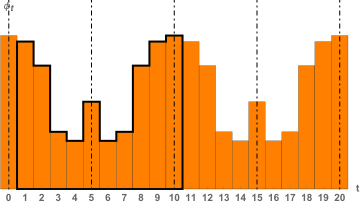
\includegraphics[width=0.40\textwidth]{HL1dLatticeStateBar4}\quad
{$(eo)$}
\includegraphics[width=0.40\textwidth]{HL1dLatticeStateBar3}
%\caption{\label{fig:symmLattStates}
  \end{center}

$(n)$ {\em no reflection symmetry:}
    $H_{5}$ invariant period-5 {\lattstate}

$(o)$ {\em odd period, symmetric:}
    an $H_{9,8}$ invariant period-9

$(ee)$ {\em even period, even symmetric:}
    $H_{10,0}$  invariant period-10

$(eo)$ {\em even period, odd symmetric:}
    $H_{10,9}$  invariant period-10
\end{frame} %%%%%%%%%%%%%%%%%%%%%%%%%%%%%%%%%%%%%%%%%%%%%%

\begin{frame} {example : 5-period Bravais lattice site, with reflection}
    \begin{block}{scalar \emph{field} $\ssp(x)$}
\begin{center}
            \begin{minipage}[c]{0.32\textwidth}\begin{center}
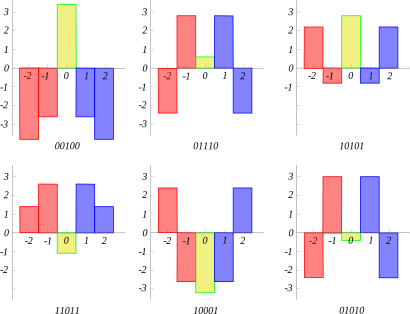
\includegraphics[width=0.55\textwidth]{PChenlatt5cyc} % from HL1dLattRefl0.svg
            \end{center}
            \end{minipage}
            \hspace{2ex}
            \begin{minipage}[c]{0.46\textwidth}
\henlatt\ period-5\\
{\lattstate}
$
\ssp_{-2} \ssp_{-1} {\ssp_0}\,\ssp_1 \ssp_2
$

\beq
\ssp_{i} = \ssp_{i+5}
    \,, \quad
\ssp_{-i} = \ssp_{i}
\,.
\ee{symmCycD5bcs}

            \end{minipage}
\end{center}
reflection symmetric; fixed lattice field ${\ssp_0}$ colored gold
%\label{fig:PChenlatt5cyc} % started with {SVW5CycHamHen}
    \end{block}
\beq
\begin{aligned}
    -S'[\ssp_{0}] + 2 \ssp_1 = -m_0 \\
\ssp_0 -S'[\ssp_{1}] +\ssp_2 = -m_1 \\
\ssp_1 -S'[\ssp_{2}] +\ssp_2 = -m_2
\end{aligned}
\ee{symmCycD5eqs} % from {HLsymmCycD5eqs}
with a 3\dmn\ {\jacobianOrb}
\bea
\jMorb &=&
\left(\begin{array}{ccc}
-{s}_0 & 2 & 0 \\
 1 &-{s}_1 & 1 \\
 0 & 1 &-{s}_2+1
\end{array}\right)
%\label{OrbJacobianD5} % from {HLOrbJacobianD5}
\eea

\end{frame} %%%%%%%%%%%%%%%%%%%%%%%%%%%%%%%%%%%%%%%%%%%%%%

\begin{frame} {what neither Fritz nor Predrag understood that day in 1988}

{\po\ theory, version (1) : counting {\lattstate}s}\footfullcite{Lind96}

\begin{block}{Lind zeta function}
\beq
\zeta_{Lind}(t) =
\exp \left( \sum_{H} \;
            \frac{N_{H}}{|\Group/{H}|}t^{|\Group/H|}
      \right)
\ee{LC21Ryu17eq:1.3}
sum is over all subgroups $H$ of space group $\Group$
\\
$N_{H}$ is the number of fixed points of $H$
\\
$|\Group/{H}|$ is the number of states in $H$ orbit
\end{block}
        \begin{enumerate}
              \item
Lind zeta function counts group {\color{blue} orbits}, one per each set of equivalent
{\lattstate}s
            \end{enumerate}
\end{frame} %%%%%%%%%%%%%%%%%%%%%%%%%%%%%%%%%%%%%%%%%%%%%%

\begin{frame} {what neither Fritz nor Predrag understood that day in 1988}

{\po\ theory, version (1) :
\\
counting {\lattstate}s} for reflection-symmetric systems%
\footfullcite{ArtMaz65}${}^,$\footfullcite{KiLePa03}

\begin{block}{Kim-Lee-Park zeta function}
\beq
\zeta_{\Refl}(t) = \sqrt{\zeta_{top}(t^2)} \; e^{h(t)},
\ee{LC21Ryu17eq:2.1}
where $\zeta_{top}$ is the
Artin-Mazur zeta function,
and the counts of the 3 kinds of symmetric orbits are
\beq
h(t) = \sum_{m=1}^{\infty} \left\{
       N_{2m-1, 0}\,t^{2m-1}
       + \left(N_{2m,0}+N_{2m,1}\right)\,\frac{ t^{2m}}{2}
                               \right\}
\ee{LC21Ryu17eq:2.11}
\end{block}
\end{frame} %%%%%%%%%%%%%%%%%%%%%%%%%%%%%%%%%%%%%%%%%%%%%%

\begin{frame}{the goal was (and still is)}
\vfill

\begin{center}
{\Large build
\\
a chaotic field theory
\medskip

from
\\
the simplest chaotic blocks}
\end{center}

\vfill
using
\begin{itemize}
  \item
\textcolor{blue}{time invariance}
  \item
\textcolor{blue}{space invariance}
\end{itemize}
 of the defining partial differential equations
\end{frame} %%%%%%%%%%%%%%%%%%%%%%%%%%%%%%%%%%%%%%%%%%%%%%

\begin{frame}{take-home :   }
\begin{center}
            \begin{minipage}[c]{0.40\textwidth}\begin{center}
{\color{purple}harmonic} field theory
\bigskip

\includegraphics[width=0.85\textwidth]{mattressSpring}\\
{\color{blue}tight-binding} model
            \end{center}\end{minipage}
            \hspace{2ex}
            \begin{minipage}[c]{0.46\textwidth}\begin{center}
{\color{purple}chaotic} field theory\\
\bigskip
\bigskip
\bigskip

\includegraphics[width=1.0\textwidth]{flagellum1}\\
\bigskip

herding cats
            \end{center}\end{minipage}
\end{center}
\end{frame}%%%%%%%%%%%%%%%%%%%%%%%%%%%%%%%%%%%%%%%%%%%%%%

\begin{frame} {what Eugene and Predrag still do not understand today}
  \begin{enumerate}
              \item
solved so far only 1\dmn\ {\color{orange}spatio}{temporal} lattice,
\\
point group \Dn{1} (!)
              \item
all time-reversal symmetric systems should be analyzed this way
              \item
all dynamical systems should be solved on reciprocal lattice (?!)
              \item
for 2\dmn\ \spt\ chaotic field theory,
\\
still have to do this for square lattice point group \Dn{4}
              \item
then, solve the problem of turbulence \\
(Navier-Stokes, Yang-Mills, general relativity)
   \end{enumerate}
\end{frame} %%%%%%%%%%%%%%%%%%%%%%%%%%%%%%%%%%%%%%%%%%%%%%

%\begin{frame} {XXX}
%\end{frame} %%%%%%%%%%%%%%%%%%%%%%%%%%%%%%%%%%%%%%%%%%%%%%
%
%\begin{frame} {XXX}
%\end{frame} %%%%%%%%%%%%%%%%%%%%%%%%%%%%%%%%%%%%%%%%%%%%%%
%
%\begin{frame} {XXX}
%\end{frame} %%%%%%%%%%%%%%%%%%%%%%%%%%%%%%%%%%%%%%%%%%%%%%
%
%\begin{frame} {XXX}
%\end{frame} %%%%%%%%%%%%%%%%%%%%%%%%%%%%%%%%%%%%%%%%%%%%%%
%
%
%

\begin{frame} {"Quantum Chaos, Graphs and Nodal Domains"\\
                Weizmann Inst., September 2016}
\begin{center}
\hfill\includegraphics[width=0.95\textheight]{IMG_3165}
\end{center}

Bye Fritz Haake. You were so brave.
\end{frame} %%%%%%%%%%%%%%%%%%%%%%%%%%%%%%%%%%%%%%%%%%%%%%

%%% #######################################

\end{document}
